\documentclass{standalone}
% Load any packages needed for this document
\begin{document}
% Your document or picture
\chapter{Выделение структур английского языка удовлетворяющих перечислениям}%Исследование грамматики английского языка}
\ttl
\section{Определение структур языка являющихся перечислениями}
\par Для построения модели перечисления в контексте естественного языка, необходимо определить структуры языка подходящие на роль перечислений. В естественных языках перечислениями являются однородные члены предложения, а также сложно сочиненные члены предложения.
\par В английском языке существуют следующие однородные члены предложения:
\begin{enumerate}
    \item сказуемые;
    \item подлежащие;
    \item определения;
    \item дополнения;
    \item обстоятельства.
\end{enumerate}
\par Рассмотрение каждой структуры в отдельности позволит построить модель перечисления на естественном языке, и выработать алгоритм определения перечислений для естественного языка.
\subsection{Сказуемое} % (fold)
% описание
% пример
% используемое правило
% 
\par Сказуемое является главным членом двусоставного предложения, обозначающим действие или признак того, что выражено подлежащим.
\par Сказуемое имеет лексическое значение (именует то, что сообщается о реалии, названной в подлежащем) и грамматическое значение (характеризует высказывание с точки зрения реальности или ирреальности и соотнесенности высказывания с моментом речи, что выражается формами наклонения глагола, а в изъявительном наклонении — и времени).
\par Рассмотрим как пример следующее предложение: <<We went to the cafe and buy a cup of coffee.>>. Для большей наглядности используем изображение ~\ref{skazuemoe}.
\begin{figure}
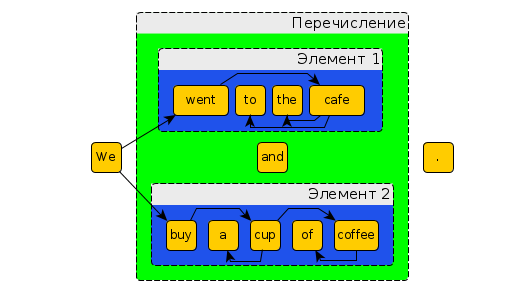
\includegraphics[width=\textwidth]{images/sentences2.png}
\label{skazuemoe}
\caption{Предложение с однородными сказуемыми, осложнеными зависимыми членами предложения}
\end{figure}
\begin{figure}
    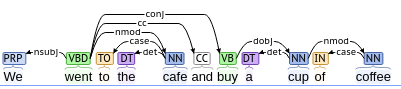
\includegraphics[width=\textwidth]{images/sentences21.png}
\label{skazuemoe2}
\caption{Предложение с однородными сказуемыми, осложнеными зависимыми членами предложения}
\end{figure}
\par На рисунке ~\ref{skazuemoe} выделены элементы перечисления, и стрелками показаны важные для нас отношения членов предложения. От подлежащего <<We>> две стрелки идут к однородным членам <<went>>  и <<buy>> , осложненым обстоятельством места и дополнением связи с ними также показаны на рисунке. На рисунке ~\ref{skazuemoe2} представлено дерево построенное Стенфорским парсером для данного предложения, оно выглядит иначе, основынм отличием является то что он подлежащего построена связь только к первому однородному сказуемому, в свою очередь существует связь соединяющая однородные члены между собой. Специфика построения синтаксических деревьев будет учтена при создании модели перечисления.
\subsection{Подлежащее} % (fold)
\par Подлежащее называет то, о ком или о чём говорится в предложении. Подлежащие не разрывно связано со сказуемым. Рассмотрим в качестве примера следующее предложение: <<Hot coffee and green tea the are best monday morning drinks.>>. Связи элементов представлены на рисунке ~\ref{podlezhachie}, в данном случае два однородных подлежащих <<coffee>> и <<tea>> , осложненные определениями, связаны со сказуемым <<are>> . На рисунке ~\ref{podlezhachie2} изображено посттроенное дерево. Тут как и в первом случае присутсвуют отличия, демонстрирующие отличие логического подхода построения связей между элементами от лингвистического подхода синтаксического подхода. Данное различие так же необходимо учесть при создании модели.

\begin{figure}[!ht]
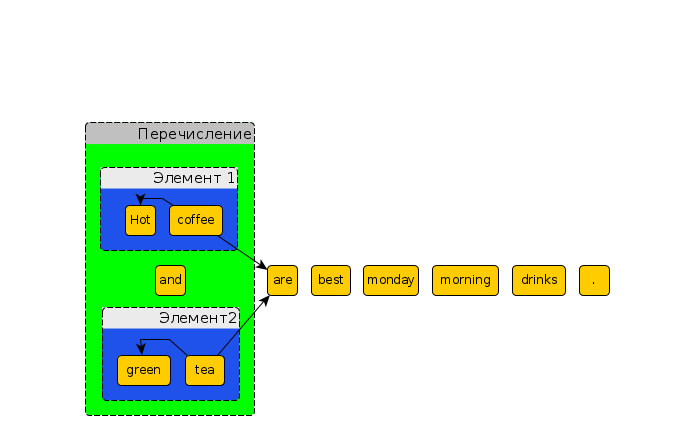
\includegraphics[width=\textwidth]{images/sentences1.png}
\label{podlezhachie}
\caption{Предложение с однородными подлежащими, осложнеными зависимыми членами предложения}
\end{figure}
\begin{figure}[!ht]
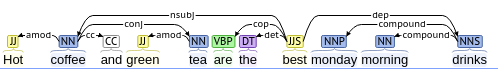
\includegraphics[width=\textwidth]{images/sentences11.png}
\label{podlezhachie2}
\caption{Предложение с однородными подлежащими, осложнеными зависимыми членами предложения}
\end{figure}
\newpage
\subsection{Определение} % (fold)
\par Определение — второстепенный член предложения, обозначающий признак, качество, свойство предмета. Рассмотрим на примере следующего предложения <<The weather today is a little cloudy, extremely raining, freezing-cold and densy foggy.>>. На рисунке ~\ref{opredelenie} представлены члены предложения и важные для исследования связи между ними. Связи отвечающие за однородные члены идут от лексеммы <<weather>> к лексеммам являющихся определениями <<cloudy>>, <<raining>>, <<freezing-cold>> и <<foggy>>, так же как и в примерах выше присутствуют зависимые лексемы. Результат определния связей между лексемами представлен на рисунке ~\ref{opredelenie2}, прослеживается общая для каждого из примеров логика, что связь между подлежащим и однородными определениями парсер представляет в виде связей двух видов: 
\begin{enumerate}
    \item связь подлежащего и первого из однородных определений;
    \item связи между первым и остальными определниями.
\end{enumerate}

\begin{figure}[!ht]
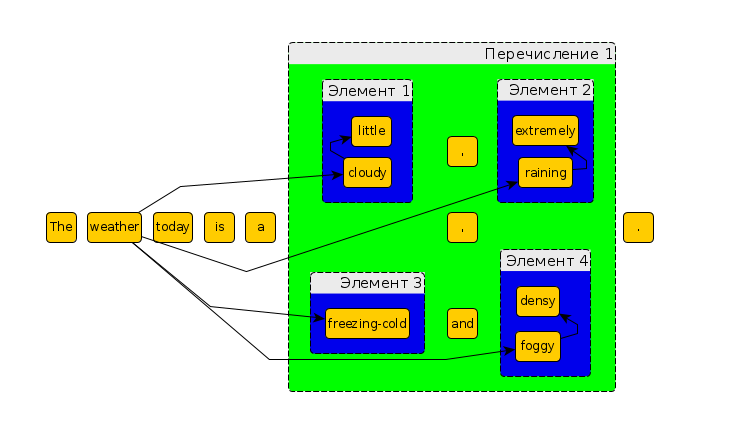
\includegraphics[width=\textwidth]{images/sentences7.png}
\label{opredelenie}
\caption{Предложение с однородными определениями}
\end{figure}
\begin{figure}[!ht]
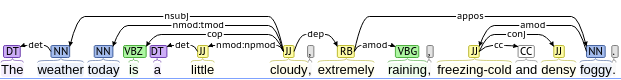
\includegraphics[width=\textwidth]{images/sentences71.png}
\label{opredelenie2}
\caption{Предложение с однородными определениями}
\end{figure}
\subsection{Дополнение} % (fold)
% описание
% пример
% используемое правило
%
Дополнение — второстепенный член предложения, выраженный существительным или местоименным существительным. Дополнение обозначает предмет или лицо, являющееся объектом действия, выраженного сказуемым.
We need your first and last names, back-white photo and home and mobile number.
\begin{figure}[!ht]
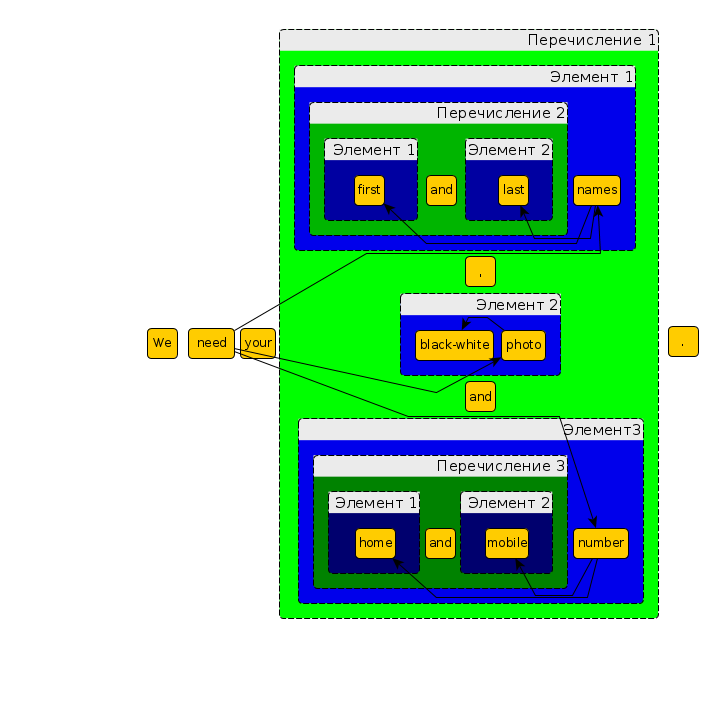
\includegraphics[width=\textwidth]{images/sentences6.png}
\label{obstoyatelstvo}
\caption{Предложение с однородными сказуемыми, осложнеными зависимыми лексемами}
\end{figure}
\newpage
\subsection{Обстоятельства} % (fold)
% описание
% пример
% используемое правило
%
I go to the cinema, cafe and to the park.
\begin{figure}[!ht]
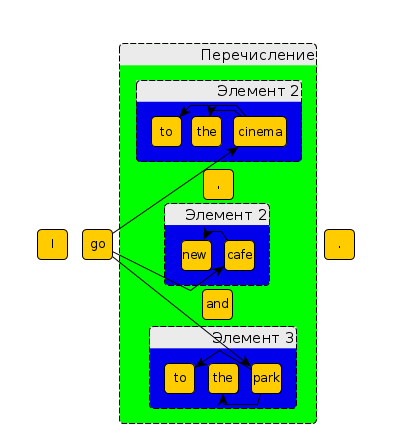
\includegraphics[width=\textwidth]{images/sentences3.png}
\label{obstoyatelstvo}
\caption{Предложение с однородными сказуемыми, осложнеными зависимыми лексемами 1}
\end{figure}
\newpage
\subsection{Сложносочиненые предложения} % (fold)
% описание
% пример
% используемое правило
%
I see a big group of people which contains three subgroups: children, women and men, who were dressed in blue overalls or strange suits with red and green lines.

\begin{figure}[!ht]
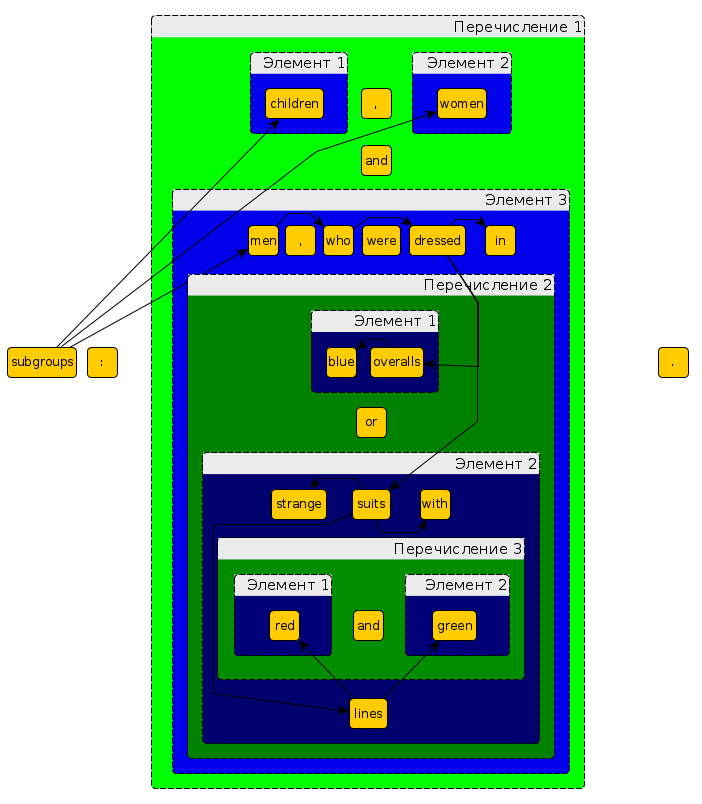
\includegraphics[width=\textwidth]{images/sentences5.png}
\label{sss}
\caption{Предложение с однородными сказуемыми, осложнеными зависимыми лексемами}
\end{figure}
\newpage
\section{Построение модели}
%
\par 
\end{document}
